\documentclass[
	letterpaper, % Paper size, specify a4paper (A4) or letterpaper (US letter)
	10pt, % Default font size, specify 10pt, 11pt or 12pt
]{CSUniSchoolLabReport}

%----------------------------------------------------------------------------------------
%	REPORT INFORMATION
%----------------------------------------------------------------------------------------

\title{Experiment Eight\\ Fundamentals of Electromagnetics Lab \\ EECE2530/1} % Report title

\author{Michael \textsc{Brodskiy}\\ \small \href{mailto:Brodskiy.M@Northeastern.edu}{Brodskiy.M@Northeastern.edu}}

\date{December 7, 2023} % Date of the report

%----------------------------------------------------------------------------------------


\begin{document}

\maketitle % Insert the title, author and date using the information specified above

\begin{center}
	\begin{tabular}{l r}
		Date Performed: & November 29, 2023 \\ % Date the experiment was performed
        Partners: & Manas \textsc{Mahajan} \& Priyam \textsc{Modi} \\ % Partner names
		Instructor: & Professor \textsc{Marengo-Fuentes} \\ % Instructor/supervisor
        TAs: & Nicolas \textsc{Casilli} \& Farah \textsc{Ben Ayed} \\ % Teachers Assistants 
	\end{tabular}
\end{center}

\newpage

\begin{abstract}

  The goal of this laboratory experiment was to verify the accuracy of Malus' Law through implementations of linear polarizers of varying length in tandem with a power meter. We begin by performing theoretical calculations using Malus' law, and then test these values against experimental values obtained using quarter-wave and half-wave polarizers.

\end{abstract}

\begin{flushleft}

  \textsc{Keywords:} \underline{Malus' Law}, \underline{linear polarizer}, \underline{power meter}, \underline{quarter-wave}, \underline{half-wave}

\end{flushleft}

\newpage

\section{Equipment}

\hspace{.5 in} Available equipment included:\\

\begin{itemize}

  \item 2 Polarizers:

    \begin{itemize}

      \item 1 Half-wave Plate

      \item 1 Quarter-wave Plate

    \end{itemize}

  \item Power meter

  \item Samples to measure optical properties:

    \begin{itemize}

      \item Transparent acrylic (plexiglass) plate

      \item Microscope slide glass

      \item Plastic plate with printed characters

    \end{itemize}

\end{itemize}

\section{Introduction \& Objectives}

We begin by performing calculations using Malus' Law to create a table of theoretical values. We find the theoretical relative intensity ($I/I_o$) using certain angle values. This generates the following plot:

\begin{figure}[h!]
  \centering
  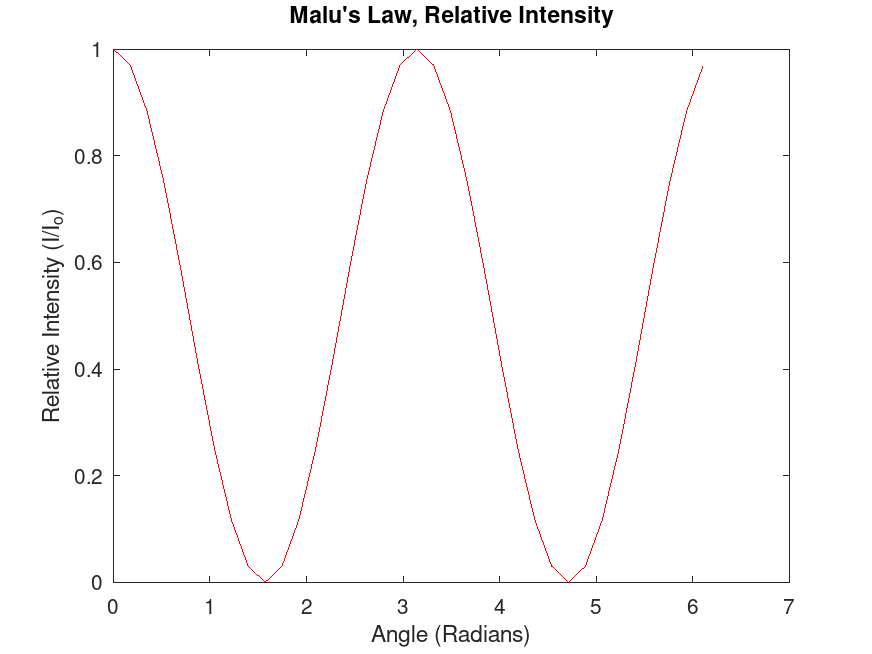
\includegraphics[width=.9\textwidth]{Figures/Lab Eight/MaluTheor.png}
  \caption{Theoretical Intensity Values}
  \label{fig:1}
\end{figure}

After this, experimental values were obtained using both quarter-wave and half-wave polarizers.

\section{Results \& Analysis} 

The experimental values obtained for the half-wave polarizer may be tabulated as follows:

\begin{multicols}{3}

\begin{center}
  \begin{tabular}[H]{|c|c|}
    \hline
    $\theta[^{\circ}]$ & Relative $I$\\
    \hline
    0 & .05531\\
    \hline
    10 & .009469\\
    \hline
    20 & .016991\\
    \hline
    30 & .079735\\
    \hline
    40 & .17699\\
    \hline
    50 & .32035\\
    \hline
    60 & .47257\\
    \hline
    70 & .62301\\
    \hline
    80 & .73982\\
    \hline
    90 & .82035\\
    \hline
    100 & .85044\\
    \hline
    110 & .83451\\
    \hline
  \end{tabular}
\end{center}

\begin{center}
  \begin{tabular}[H]{|c|c|}
    \hline
    $\theta[^{\circ}]$ & Relative $I$\\
    \hline
    120 & .76637\\
    \hline
    130 & .66991\\
    \hline
    140 & .53894\\
    \hline
    150 & .38496\\
    \hline
    160 & .25044\\
    \hline
    170 & .1292\\
    \hline
    180 & .037434\\
    \hline
    190 & .0061947\\
    \hline
    200 & .031858\\
    \hline
    210 & .10088\\
    \hline
    220 & .21239\\
    \hline
    230 & .36018\\
    \hline
  \end{tabular}
\end{center}

\begin{center}
  \begin{tabular}[H]{|c|c|}
    \hline
    $\theta[^{\circ}]$ & Relative $I$\\
    \hline
    240 & .52124\\
    \hline
    250 & .65133\\
    \hline
    260 & .76372\\
    \hline
    270 & .83982\\
    \hline
    280 & .85221\\
    \hline
    290 & .83274\\
    \hline
    300 & .77788\\
    \hline
    310 & .68407\\
    \hline
    320 & .53894\\
    \hline
    330 & .39381\\
    \hline
    340 & .24336\\
    \hline
    350 & .12478\\
    \hline
  \end{tabular}
\end{center}

\end{multicols}

These values then allowed us to generate the following plot:

\begin{figure}[H]
  \centering
  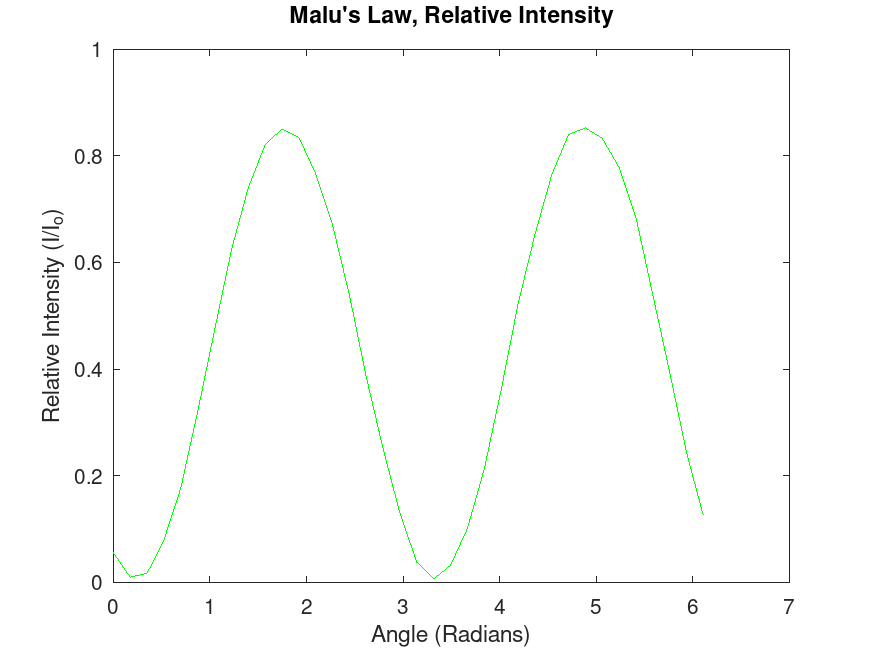
\includegraphics[width=.9\textwidth]{Figures/Lab Eight/Half-Wave.png}
  \caption{Half-Wave Plate, Experimental Values}
  \label{fig:2}
\end{figure}

The experiment was then repeated for a quarter-wave. For this, the values may be tabulated as follows:

\begin{center}
  \begin{tabular}[H]{|c|c|}
    \hline
    $\theta[^{\circ}]$ & Relative $I$\\
    \hline
    0 & .037633\\
    \hline
    10 & .0054628\\
    \hline
    20 & .022155\\
    \hline
    30 & .081184\\
    \hline
    40 & .17678\\
    \hline
    50 & .30425\\
    \hline
    60 & .43703\\
    \hline
    70 & .56525\\
    \hline
    80 & .67071\\
    \hline
    90 & .74431\\
    \hline
    100 & .77086\\
    \hline
    110 & .74962\\
    \hline
  \end{tabular}
\end{center}

\begin{center}
  \begin{tabular}[H]{|c|c|}
    \hline
    $\theta[^{\circ}]$ & Relative $I$\\
    \hline
    120 & .68665\\
    \hline
    130 & .57436\\
    \hline
    140 & .45448\\
    \hline
    150 & .30956\\
    \hline
    160 & .19651\\
    \hline
    170 & .093323\\
    \hline
    180 & .023748\\
    \hline
    190 & .0048558\\
    \hline
    200 & .031108\\
    \hline
    210 & .091047\\
    \hline
    220 & .19727\\
    \hline
    230 & .31335\\
    \hline
  \end{tabular}
\end{center}

\begin{center}
  \begin{tabular}[H]{|c|c|}
    \hline
    $\theta[^{\circ}]$ & Relative $I$\\
    \hline
    240 & .44689\\
    \hline
    250 & .5698\\
    \hline
    260 & .66844\\
    \hline
    270 & .73293\\
    \hline
    280 & .75873\\
    \hline
    290 & .73445\\
    \hline
    300 & .67754\\
    \hline
    310 & .57663\\
    \hline
    320 & .44917\\
    \hline
    330 & .32473\\
    \hline
    340 & .19803\\
    \hline
    350 & .097117\\
    \hline
  \end{tabular}
\end{center}

\end{multicols}

These values then allowed us to generate the following plot:

\begin{figure}[H]
  \centering
  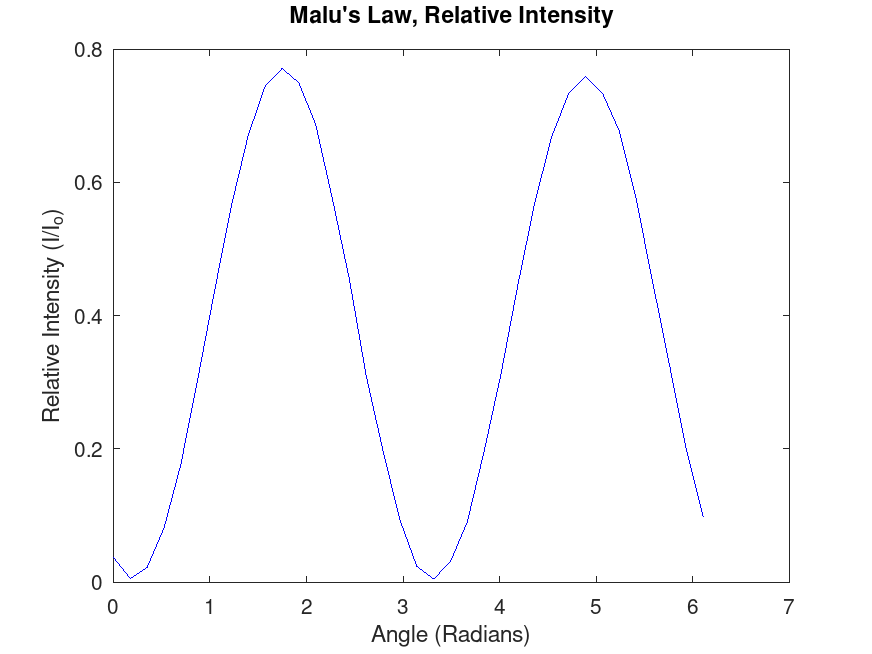
\includegraphics[width=.9\textwidth]{Figures/Lab Eight/Quar-Wave.png}
  \caption{Quarter-Wave Plate, Experimental Values}
  \label{fig:3}
\end{figure}

\section{Conclusion}

Overall, we can see that, experimentally, our results are quite similar to the theoretical expectations laid out by Malus' Law. The only (minor) difference is a phase shift; however, this is not a significant difference, as the sinusoidal pattern is key. As such, we conclude the accuracy of Malus' Law in various materials.

\end{document}
